\documentclass[../main.tex]{subfiles}

\begin{document}
\subsection{Spustenie Docker kontajnera na Azure Cloude}
Po aktivácií predplatného pre študentov služby Azure som získal prístup k Azure portalu, kde môžem umiestniť moje aplikácie, kontajnery alebo môžem vytvoriť virtuálny stroj. K službám treba pripojiť dátový priestor. Pre uchovávanie kontajnerov som si vytvoril Container Registry. Ďalšia vec, ktorú som spravil bola vytvorenie inštancie kontajnera pomocou menu v Azure portali. Mohol som si vybrať konfiguráciu podľa vlastných potrieb. Nastavil som jedno CPU jadro a 1,5 Gib RAM. Bola to jedna z najslabších možných konfigurácií. Na Obr.\ref{fig:azure_monitor} s grafmi monitorovacieho nástroja Azure je vidieť, že súčasná konfigurácia je pre túto kontajnerizovanú aplikáciu postačujúca s dostatočnou rezervou.
\begin{wrapfigure}{l}[-8mm]{0.6\textwidth}
    \centering
    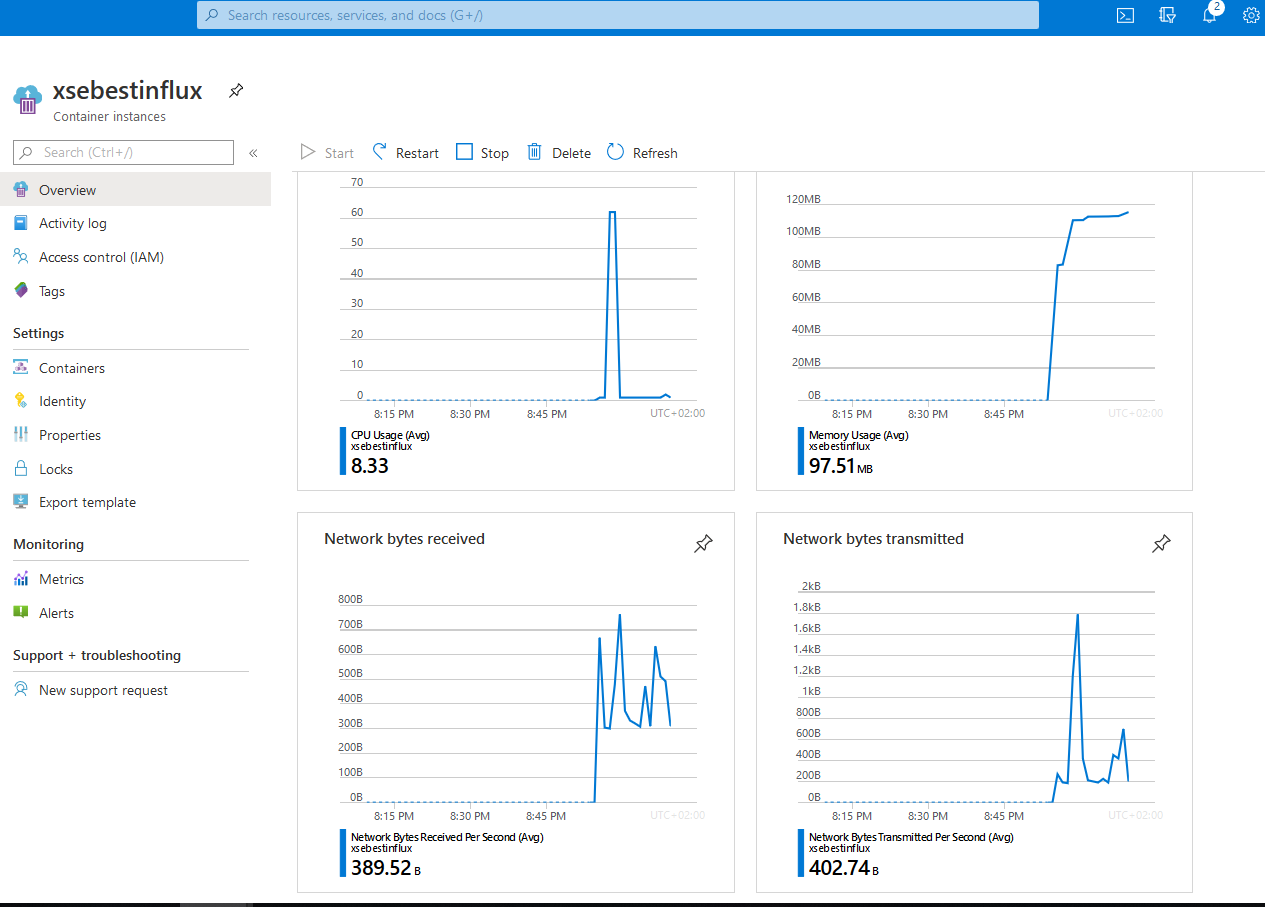
\includegraphics[width = 0.56\textwidth]{images/azure_monitor.png}
    \caption{Záťaž pre inštanciu po spusteného kontajnera}
    \label{fig:azure_monitor}
\end{wrapfigure}
Podľa tohto usudzujem, že by bolo možné rozšíriť používaný Docker Image o ďalšie platformy (NodeRed, Telegraf). Podľa výpočtu na stránke Azure %\url{https://azure.microsoft.com/en-us/pricing/calculator/?service=container-instances} neviem zorazit link do riadkov
pre odhadovú cenu služby vychádza cena za takúto službu okolo 35\$ mesačne. Čo potvrdzuje aj aktuálna faktúra. Služby kontajnera som manažoval pomocou Bashu. Napríklad vytvorenie databázy v InfluxDB. Fully qualified domain name (FQDN) pre inštanciu kontajnera je
\newline\url{xsebestinflux.northeurope.azurecontainer.io}. Grafana beží na porte 3003 a InfluxDB na 8086.

\begin{figure}[h!]
    \centering
    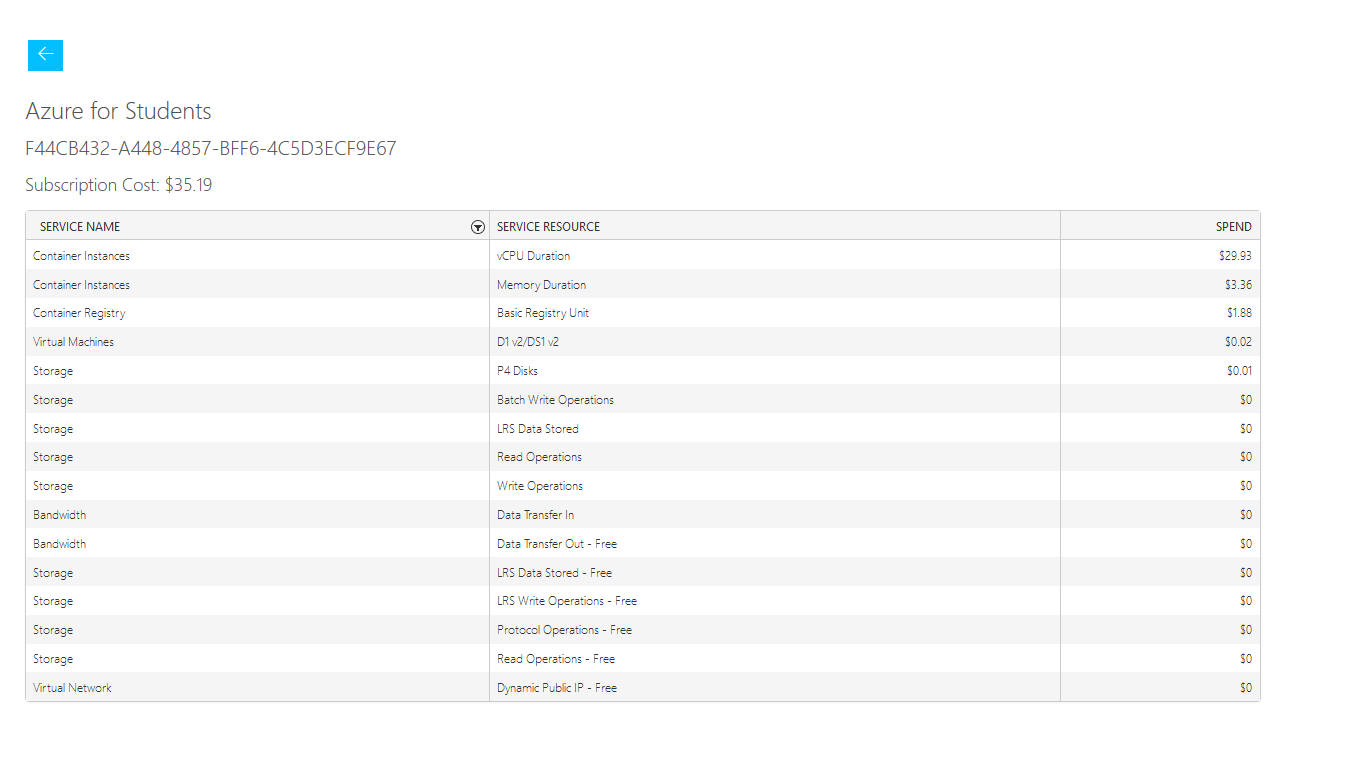
\includegraphics[width = 0.71\textwidth]{images/subscription_cost_azure.png}
    \caption{cena použitej služby Container instance}
    \label{fig:cost}
\end{figure}

\end{document}